\section{Transformée de \textsc{Laplace}} 
\label{transformee_laplace}

\todoinline{On pourrait tenter une illustration ? La transformée de Laplace d'une fonction échelon ?}
\todoarmand{J'ai proposé une illustration mais j'aimerais la compléter avec d'autres transformées de fonctions usuelles. \\
Un thème assez développé sur la transformée de Laplace : \url{https://cahier-de-prepa.fr/ecg2-saintlouis/download?id=289}
}

La transformation de \textsc{Laplace} généralise la transformation de \textsc{Fourier} qui est également utilisée pour résoudre les équations différentielles : contrairement à cette dernière, elle tient compte des conditions initiales et peut ainsi être utilisée en théorie des vibrations mécaniques ou en électricité dans l'étude des régimes forcés sans négliger le régime transitoire. De manière générale, ses propriétés vis-à-vis de la dérivation permettent un traitement plus simple de certaines équations différentielles, et elle est de ce fait très utilisée en automatique.

Dans ce type d'analyse, la transformation de \textsc{Laplace} est souvent interprétée comme un passage du domaine temps, dans lequel les entrées et sorties sont des fonctions du temps, dans le domaine des fréquences, dans lequel les mêmes entrées et sorties sont des fonctions de la \say{ fréquence } (complexe) $p$. Ainsi; il est possible d'analyser simplement l'effet du système sur l'entrée pour donner la sortie en matière d'opérations algébriques simples (cf. théorie des fonctions de transfert en électronique ou en mécanique). 

\begin{defi}{Transformée de \textsc{Laplace}}
    Pour tout fonction $f \in \mathscr{C}(\Rp, \R)$, on note, lorsqu'elle converge, 
    $$\mathscr{L}(f)(p) \defeq \int_{0}^{+ \infty} \e^{-pt} f(t) \d t.$$
    La fonction $\mathscr{L}(f)$ est la \emph{transformée de \textsc{Laplace} de f}.
\end{defi}

\marginnote[0cm]{Sources : \cite{exos_oraux} + \cite{acamanes} (Exercice cerise Ch. 12)}
% \underline{Démonstration du théorème de la valeur finale:}
% \begin{itemize}
    % \item Généralisation classique du théorème des bornes $\leadsto$ $f$ est bornée
    % \item Changement de variable: $\varphi: u \mapsto \frac{u}{p}$
    % \item Caractérisation séquentielle de la limite
    % \item Théorème de convergence dominée
% \end{itemize}

%-----------
\subsection{Exemples de transformées de Laplace}

\begin{marginfigure}[0cm]
    \centering
    %% Creator: Matplotlib, PGF backend
%%
%% To include the figure in your LaTeX document, write
%%   \input{<filename>.pgf}
%%
%% Make sure the required packages are loaded in your preamble
%%   \usepackage{pgf}
%%
%% Also ensure that all the required font packages are loaded; for instance,
%% the lmodern package is sometimes necessary when using math font.
%%   \usepackage{lmodern}
%%
%% Figures using additional raster images can only be included by \input if
%% they are in the same directory as the main LaTeX file. For loading figures
%% from other directories you can use the `import` package
%%   \usepackage{import}
%%
%% and then include the figures with
%%   \import{<path to file>}{<filename>.pgf}
%%
%% Matplotlib used the following preamble
%%   
%%   \usepackage{fontspec}
%%   \setmainfont{DejaVuSerif.ttf}[Path=\detokenize{/home/wayoff/.pyenv/versions/3.8.10/lib/python3.8/site-packages/matplotlib/mpl-data/fonts/ttf/}]
%%   \setsansfont{DejaVuSans.ttf}[Path=\detokenize{/home/wayoff/.pyenv/versions/3.8.10/lib/python3.8/site-packages/matplotlib/mpl-data/fonts/ttf/}]
%%   \setmonofont{DejaVuSansMono.ttf}[Path=\detokenize{/home/wayoff/.pyenv/versions/3.8.10/lib/python3.8/site-packages/matplotlib/mpl-data/fonts/ttf/}]
%%   \makeatletter\@ifpackageloaded{underscore}{}{\usepackage[strings]{underscore}}\makeatother
%%
\begingroup%
\makeatletter%
\begin{pgfpicture}%
\pgfpathrectangle{\pgfpointorigin}{\pgfqpoint{3.000000in}{6.000000in}}%
\pgfusepath{use as bounding box, clip}%
\begin{pgfscope}%
\pgfsetbuttcap%
\pgfsetmiterjoin%
\definecolor{currentfill}{rgb}{1.000000,1.000000,1.000000}%
\pgfsetfillcolor{currentfill}%
\pgfsetlinewidth{0.000000pt}%
\definecolor{currentstroke}{rgb}{1.000000,1.000000,1.000000}%
\pgfsetstrokecolor{currentstroke}%
\pgfsetdash{}{0pt}%
\pgfpathmoveto{\pgfqpoint{0.000000in}{0.000000in}}%
\pgfpathlineto{\pgfqpoint{3.000000in}{0.000000in}}%
\pgfpathlineto{\pgfqpoint{3.000000in}{6.000000in}}%
\pgfpathlineto{\pgfqpoint{0.000000in}{6.000000in}}%
\pgfpathlineto{\pgfqpoint{0.000000in}{0.000000in}}%
\pgfpathclose%
\pgfusepath{fill}%
\end{pgfscope}%
\begin{pgfscope}%
\pgfsetbuttcap%
\pgfsetmiterjoin%
\definecolor{currentfill}{rgb}{1.000000,1.000000,1.000000}%
\pgfsetfillcolor{currentfill}%
\pgfsetlinewidth{0.000000pt}%
\definecolor{currentstroke}{rgb}{0.000000,0.000000,0.000000}%
\pgfsetstrokecolor{currentstroke}%
\pgfsetstrokeopacity{0.000000}%
\pgfsetdash{}{0pt}%
\pgfpathmoveto{\pgfqpoint{0.530032in}{3.496603in}}%
\pgfpathlineto{\pgfqpoint{2.850000in}{3.496603in}}%
\pgfpathlineto{\pgfqpoint{2.850000in}{5.850000in}}%
\pgfpathlineto{\pgfqpoint{0.530032in}{5.850000in}}%
\pgfpathlineto{\pgfqpoint{0.530032in}{3.496603in}}%
\pgfpathclose%
\pgfusepath{fill}%
\end{pgfscope}%
\begin{pgfscope}%
\pgfpathrectangle{\pgfqpoint{0.530032in}{3.496603in}}{\pgfqpoint{2.319968in}{2.353397in}}%
\pgfusepath{clip}%
\pgfsetrectcap%
\pgfsetroundjoin%
\pgfsetlinewidth{0.803000pt}%
\definecolor{currentstroke}{rgb}{0.690196,0.690196,0.690196}%
\pgfsetstrokecolor{currentstroke}%
\pgfsetdash{}{0pt}%
\pgfpathmoveto{\pgfqpoint{1.900922in}{3.496603in}}%
\pgfpathlineto{\pgfqpoint{1.900922in}{5.850000in}}%
\pgfusepath{stroke}%
\end{pgfscope}%
\begin{pgfscope}%
\pgfsetbuttcap%
\pgfsetroundjoin%
\definecolor{currentfill}{rgb}{0.000000,0.000000,0.000000}%
\pgfsetfillcolor{currentfill}%
\pgfsetlinewidth{0.803000pt}%
\definecolor{currentstroke}{rgb}{0.000000,0.000000,0.000000}%
\pgfsetstrokecolor{currentstroke}%
\pgfsetdash{}{0pt}%
\pgfsys@defobject{currentmarker}{\pgfqpoint{0.000000in}{-0.048611in}}{\pgfqpoint{0.000000in}{0.000000in}}{%
\pgfpathmoveto{\pgfqpoint{0.000000in}{0.000000in}}%
\pgfpathlineto{\pgfqpoint{0.000000in}{-0.048611in}}%
\pgfusepath{stroke,fill}%
}%
\begin{pgfscope}%
\pgfsys@transformshift{1.900922in}{3.496603in}%
\pgfsys@useobject{currentmarker}{}%
\end{pgfscope}%
\end{pgfscope}%
\begin{pgfscope}%
\definecolor{textcolor}{rgb}{0.000000,0.000000,0.000000}%
\pgfsetstrokecolor{textcolor}%
\pgfsetfillcolor{textcolor}%
\pgftext[x=1.900922in,y=3.399381in,,top]{\color{textcolor}\sffamily\fontsize{10.000000}{12.000000}\selectfont c}%
\end{pgfscope}%
\begin{pgfscope}%
\definecolor{textcolor}{rgb}{0.000000,0.000000,0.000000}%
\pgfsetstrokecolor{textcolor}%
\pgfsetfillcolor{textcolor}%
\pgftext[x=1.690016in,y=3.209413in,,top]{\color{textcolor}\sffamily\fontsize{10.000000}{12.000000}\selectfont \(\displaystyle t\)}%
\end{pgfscope}%
\begin{pgfscope}%
\pgfpathrectangle{\pgfqpoint{0.530032in}{3.496603in}}{\pgfqpoint{2.319968in}{2.353397in}}%
\pgfusepath{clip}%
\pgfsetrectcap%
\pgfsetroundjoin%
\pgfsetlinewidth{0.803000pt}%
\definecolor{currentstroke}{rgb}{0.690196,0.690196,0.690196}%
\pgfsetstrokecolor{currentstroke}%
\pgfsetdash{}{0pt}%
\pgfpathmoveto{\pgfqpoint{0.530032in}{3.603576in}}%
\pgfpathlineto{\pgfqpoint{2.850000in}{3.603576in}}%
\pgfusepath{stroke}%
\end{pgfscope}%
\begin{pgfscope}%
\pgfsetbuttcap%
\pgfsetroundjoin%
\definecolor{currentfill}{rgb}{0.000000,0.000000,0.000000}%
\pgfsetfillcolor{currentfill}%
\pgfsetlinewidth{0.803000pt}%
\definecolor{currentstroke}{rgb}{0.000000,0.000000,0.000000}%
\pgfsetstrokecolor{currentstroke}%
\pgfsetdash{}{0pt}%
\pgfsys@defobject{currentmarker}{\pgfqpoint{-0.048611in}{0.000000in}}{\pgfqpoint{-0.000000in}{0.000000in}}{%
\pgfpathmoveto{\pgfqpoint{-0.000000in}{0.000000in}}%
\pgfpathlineto{\pgfqpoint{-0.048611in}{0.000000in}}%
\pgfusepath{stroke,fill}%
}%
\begin{pgfscope}%
\pgfsys@transformshift{0.530032in}{3.603576in}%
\pgfsys@useobject{currentmarker}{}%
\end{pgfscope}%
\end{pgfscope}%
\begin{pgfscope}%
\definecolor{textcolor}{rgb}{0.000000,0.000000,0.000000}%
\pgfsetstrokecolor{textcolor}%
\pgfsetfillcolor{textcolor}%
\pgftext[x=0.344444in, y=3.550814in, left, base]{\color{textcolor}\sffamily\fontsize{10.000000}{12.000000}\selectfont 0}%
\end{pgfscope}%
\begin{pgfscope}%
\pgfpathrectangle{\pgfqpoint{0.530032in}{3.496603in}}{\pgfqpoint{2.319968in}{2.353397in}}%
\pgfusepath{clip}%
\pgfsetrectcap%
\pgfsetroundjoin%
\pgfsetlinewidth{0.803000pt}%
\definecolor{currentstroke}{rgb}{0.690196,0.690196,0.690196}%
\pgfsetstrokecolor{currentstroke}%
\pgfsetdash{}{0pt}%
\pgfpathmoveto{\pgfqpoint{0.530032in}{5.743027in}}%
\pgfpathlineto{\pgfqpoint{2.850000in}{5.743027in}}%
\pgfusepath{stroke}%
\end{pgfscope}%
\begin{pgfscope}%
\pgfsetbuttcap%
\pgfsetroundjoin%
\definecolor{currentfill}{rgb}{0.000000,0.000000,0.000000}%
\pgfsetfillcolor{currentfill}%
\pgfsetlinewidth{0.803000pt}%
\definecolor{currentstroke}{rgb}{0.000000,0.000000,0.000000}%
\pgfsetstrokecolor{currentstroke}%
\pgfsetdash{}{0pt}%
\pgfsys@defobject{currentmarker}{\pgfqpoint{-0.048611in}{0.000000in}}{\pgfqpoint{-0.000000in}{0.000000in}}{%
\pgfpathmoveto{\pgfqpoint{-0.000000in}{0.000000in}}%
\pgfpathlineto{\pgfqpoint{-0.048611in}{0.000000in}}%
\pgfusepath{stroke,fill}%
}%
\begin{pgfscope}%
\pgfsys@transformshift{0.530032in}{5.743027in}%
\pgfsys@useobject{currentmarker}{}%
\end{pgfscope}%
\end{pgfscope}%
\begin{pgfscope}%
\definecolor{textcolor}{rgb}{0.000000,0.000000,0.000000}%
\pgfsetstrokecolor{textcolor}%
\pgfsetfillcolor{textcolor}%
\pgftext[x=0.344444in, y=5.690266in, left, base]{\color{textcolor}\sffamily\fontsize{10.000000}{12.000000}\selectfont 1}%
\end{pgfscope}%
\begin{pgfscope}%
\pgfpathrectangle{\pgfqpoint{0.530032in}{3.496603in}}{\pgfqpoint{2.319968in}{2.353397in}}%
\pgfusepath{clip}%
\pgfsetrectcap%
\pgfsetroundjoin%
\pgfsetlinewidth{1.505625pt}%
\definecolor{currentstroke}{rgb}{0.121569,0.466667,0.705882}%
\pgfsetstrokecolor{currentstroke}%
\pgfsetdash{}{0pt}%
\pgfpathmoveto{\pgfqpoint{0.635485in}{3.603576in}}%
\pgfpathlineto{\pgfqpoint{1.900078in}{3.603576in}}%
\pgfpathlineto{\pgfqpoint{1.902189in}{5.743027in}}%
\pgfpathlineto{\pgfqpoint{2.744547in}{5.743027in}}%
\pgfpathlineto{\pgfqpoint{2.744547in}{5.743027in}}%
\pgfusepath{stroke}%
\end{pgfscope}%
\begin{pgfscope}%
\pgfsetrectcap%
\pgfsetmiterjoin%
\pgfsetlinewidth{0.803000pt}%
\definecolor{currentstroke}{rgb}{0.000000,0.000000,0.000000}%
\pgfsetstrokecolor{currentstroke}%
\pgfsetdash{}{0pt}%
\pgfpathmoveto{\pgfqpoint{0.530032in}{3.496603in}}%
\pgfpathlineto{\pgfqpoint{0.530032in}{5.850000in}}%
\pgfusepath{stroke}%
\end{pgfscope}%
\begin{pgfscope}%
\pgfsetrectcap%
\pgfsetmiterjoin%
\pgfsetlinewidth{0.803000pt}%
\definecolor{currentstroke}{rgb}{0.000000,0.000000,0.000000}%
\pgfsetstrokecolor{currentstroke}%
\pgfsetdash{}{0pt}%
\pgfpathmoveto{\pgfqpoint{2.850000in}{3.496603in}}%
\pgfpathlineto{\pgfqpoint{2.850000in}{5.850000in}}%
\pgfusepath{stroke}%
\end{pgfscope}%
\begin{pgfscope}%
\pgfsetrectcap%
\pgfsetmiterjoin%
\pgfsetlinewidth{0.803000pt}%
\definecolor{currentstroke}{rgb}{0.000000,0.000000,0.000000}%
\pgfsetstrokecolor{currentstroke}%
\pgfsetdash{}{0pt}%
\pgfpathmoveto{\pgfqpoint{0.530032in}{3.496603in}}%
\pgfpathlineto{\pgfqpoint{2.850000in}{3.496603in}}%
\pgfusepath{stroke}%
\end{pgfscope}%
\begin{pgfscope}%
\pgfsetrectcap%
\pgfsetmiterjoin%
\pgfsetlinewidth{0.803000pt}%
\definecolor{currentstroke}{rgb}{0.000000,0.000000,0.000000}%
\pgfsetstrokecolor{currentstroke}%
\pgfsetdash{}{0pt}%
\pgfpathmoveto{\pgfqpoint{0.530032in}{5.850000in}}%
\pgfpathlineto{\pgfqpoint{2.850000in}{5.850000in}}%
\pgfusepath{stroke}%
\end{pgfscope}%
\begin{pgfscope}%
\pgfsetbuttcap%
\pgfsetmiterjoin%
\definecolor{currentfill}{rgb}{1.000000,1.000000,1.000000}%
\pgfsetfillcolor{currentfill}%
\pgfsetfillopacity{0.800000}%
\pgfsetlinewidth{1.003750pt}%
\definecolor{currentstroke}{rgb}{0.800000,0.800000,0.800000}%
\pgfsetstrokecolor{currentstroke}%
\pgfsetstrokeopacity{0.800000}%
\pgfsetdash{}{0pt}%
\pgfpathmoveto{\pgfqpoint{0.627254in}{5.529199in}}%
\pgfpathlineto{\pgfqpoint{1.586471in}{5.529199in}}%
\pgfpathquadraticcurveto{\pgfqpoint{1.614248in}{5.529199in}}{\pgfqpoint{1.614248in}{5.556977in}}%
\pgfpathlineto{\pgfqpoint{1.614248in}{5.752778in}}%
\pgfpathquadraticcurveto{\pgfqpoint{1.614248in}{5.780556in}}{\pgfqpoint{1.586471in}{5.780556in}}%
\pgfpathlineto{\pgfqpoint{0.627254in}{5.780556in}}%
\pgfpathquadraticcurveto{\pgfqpoint{0.599476in}{5.780556in}}{\pgfqpoint{0.599476in}{5.752778in}}%
\pgfpathlineto{\pgfqpoint{0.599476in}{5.556977in}}%
\pgfpathquadraticcurveto{\pgfqpoint{0.599476in}{5.529199in}}{\pgfqpoint{0.627254in}{5.529199in}}%
\pgfpathlineto{\pgfqpoint{0.627254in}{5.529199in}}%
\pgfpathclose%
\pgfusepath{stroke,fill}%
\end{pgfscope}%
\begin{pgfscope}%
\pgfsetrectcap%
\pgfsetroundjoin%
\pgfsetlinewidth{1.505625pt}%
\definecolor{currentstroke}{rgb}{0.121569,0.466667,0.705882}%
\pgfsetstrokecolor{currentstroke}%
\pgfsetdash{}{0pt}%
\pgfpathmoveto{\pgfqpoint{0.655032in}{5.668088in}}%
\pgfpathlineto{\pgfqpoint{0.793921in}{5.668088in}}%
\pgfpathlineto{\pgfqpoint{0.932810in}{5.668088in}}%
\pgfusepath{stroke}%
\end{pgfscope}%
\begin{pgfscope}%
\definecolor{textcolor}{rgb}{0.000000,0.000000,0.000000}%
\pgfsetstrokecolor{textcolor}%
\pgfsetfillcolor{textcolor}%
\pgftext[x=1.043921in,y=5.619477in,left,base]{\color{textcolor}\sffamily\fontsize{10.000000}{12.000000}\selectfont \(\displaystyle H(t - c)\)}%
\end{pgfscope}%
\begin{pgfscope}%
\pgfsetbuttcap%
\pgfsetmiterjoin%
\definecolor{currentfill}{rgb}{1.000000,1.000000,1.000000}%
\pgfsetfillcolor{currentfill}%
\pgfsetlinewidth{0.000000pt}%
\definecolor{currentstroke}{rgb}{0.000000,0.000000,0.000000}%
\pgfsetstrokecolor{currentstroke}%
\pgfsetstrokeopacity{0.000000}%
\pgfsetdash{}{0pt}%
\pgfpathmoveto{\pgfqpoint{0.530032in}{0.571603in}}%
\pgfpathlineto{\pgfqpoint{2.850000in}{0.571603in}}%
\pgfpathlineto{\pgfqpoint{2.850000in}{2.925000in}}%
\pgfpathlineto{\pgfqpoint{0.530032in}{2.925000in}}%
\pgfpathlineto{\pgfqpoint{0.530032in}{0.571603in}}%
\pgfpathclose%
\pgfusepath{fill}%
\end{pgfscope}%
\begin{pgfscope}%
\pgfpathrectangle{\pgfqpoint{0.530032in}{0.571603in}}{\pgfqpoint{2.319968in}{2.353397in}}%
\pgfusepath{clip}%
\pgfsetrectcap%
\pgfsetroundjoin%
\pgfsetlinewidth{0.803000pt}%
\definecolor{currentstroke}{rgb}{0.690196,0.690196,0.690196}%
\pgfsetstrokecolor{currentstroke}%
\pgfsetdash{}{0pt}%
\pgfpathmoveto{\pgfqpoint{0.604919in}{0.571603in}}%
\pgfpathlineto{\pgfqpoint{0.604919in}{2.925000in}}%
\pgfusepath{stroke}%
\end{pgfscope}%
\begin{pgfscope}%
\pgfsetbuttcap%
\pgfsetroundjoin%
\definecolor{currentfill}{rgb}{0.000000,0.000000,0.000000}%
\pgfsetfillcolor{currentfill}%
\pgfsetlinewidth{0.803000pt}%
\definecolor{currentstroke}{rgb}{0.000000,0.000000,0.000000}%
\pgfsetstrokecolor{currentstroke}%
\pgfsetdash{}{0pt}%
\pgfsys@defobject{currentmarker}{\pgfqpoint{0.000000in}{-0.048611in}}{\pgfqpoint{0.000000in}{0.000000in}}{%
\pgfpathmoveto{\pgfqpoint{0.000000in}{0.000000in}}%
\pgfpathlineto{\pgfqpoint{0.000000in}{-0.048611in}}%
\pgfusepath{stroke,fill}%
}%
\begin{pgfscope}%
\pgfsys@transformshift{0.604919in}{0.571603in}%
\pgfsys@useobject{currentmarker}{}%
\end{pgfscope}%
\end{pgfscope}%
\begin{pgfscope}%
\definecolor{textcolor}{rgb}{0.000000,0.000000,0.000000}%
\pgfsetstrokecolor{textcolor}%
\pgfsetfillcolor{textcolor}%
\pgftext[x=0.604919in,y=0.474381in,,top]{\color{textcolor}\sffamily\fontsize{10.000000}{12.000000}\selectfont 0}%
\end{pgfscope}%
\begin{pgfscope}%
\definecolor{textcolor}{rgb}{0.000000,0.000000,0.000000}%
\pgfsetstrokecolor{textcolor}%
\pgfsetfillcolor{textcolor}%
\pgftext[x=1.690016in,y=0.284413in,,top]{\color{textcolor}\sffamily\fontsize{10.000000}{12.000000}\selectfont \(\displaystyle p\)}%
\end{pgfscope}%
\begin{pgfscope}%
\pgfpathrectangle{\pgfqpoint{0.530032in}{0.571603in}}{\pgfqpoint{2.319968in}{2.353397in}}%
\pgfusepath{clip}%
\pgfsetrectcap%
\pgfsetroundjoin%
\pgfsetlinewidth{0.803000pt}%
\definecolor{currentstroke}{rgb}{0.690196,0.690196,0.690196}%
\pgfsetstrokecolor{currentstroke}%
\pgfsetdash{}{0pt}%
\pgfpathmoveto{\pgfqpoint{0.530032in}{0.647569in}}%
\pgfpathlineto{\pgfqpoint{2.850000in}{0.647569in}}%
\pgfusepath{stroke}%
\end{pgfscope}%
\begin{pgfscope}%
\pgfsetbuttcap%
\pgfsetroundjoin%
\definecolor{currentfill}{rgb}{0.000000,0.000000,0.000000}%
\pgfsetfillcolor{currentfill}%
\pgfsetlinewidth{0.803000pt}%
\definecolor{currentstroke}{rgb}{0.000000,0.000000,0.000000}%
\pgfsetstrokecolor{currentstroke}%
\pgfsetdash{}{0pt}%
\pgfsys@defobject{currentmarker}{\pgfqpoint{-0.048611in}{0.000000in}}{\pgfqpoint{-0.000000in}{0.000000in}}{%
\pgfpathmoveto{\pgfqpoint{-0.000000in}{0.000000in}}%
\pgfpathlineto{\pgfqpoint{-0.048611in}{0.000000in}}%
\pgfusepath{stroke,fill}%
}%
\begin{pgfscope}%
\pgfsys@transformshift{0.530032in}{0.647569in}%
\pgfsys@useobject{currentmarker}{}%
\end{pgfscope}%
\end{pgfscope}%
\begin{pgfscope}%
\definecolor{textcolor}{rgb}{0.000000,0.000000,0.000000}%
\pgfsetstrokecolor{textcolor}%
\pgfsetfillcolor{textcolor}%
\pgftext[x=0.344444in, y=0.594808in, left, base]{\color{textcolor}\sffamily\fontsize{10.000000}{12.000000}\selectfont 0}%
\end{pgfscope}%
\begin{pgfscope}%
\definecolor{textcolor}{rgb}{0.000000,0.000000,0.000000}%
\pgfsetstrokecolor{textcolor}%
\pgfsetfillcolor{textcolor}%
\pgftext[x=0.288889in,y=1.748302in,,bottom,rotate=90.000000]{\color{textcolor}\sffamily\fontsize{10.000000}{12.000000}\selectfont \(\displaystyle \mathcal{L}\{H(t - c)\}(p)\)}%
\end{pgfscope}%
\begin{pgfscope}%
\pgfpathrectangle{\pgfqpoint{0.530032in}{0.571603in}}{\pgfqpoint{2.319968in}{2.353397in}}%
\pgfusepath{clip}%
\pgfsetrectcap%
\pgfsetroundjoin%
\pgfsetlinewidth{1.505625pt}%
\definecolor{currentstroke}{rgb}{1.000000,0.647059,0.000000}%
\pgfsetstrokecolor{currentstroke}%
\pgfsetdash{}{0pt}%
\pgfpathmoveto{\pgfqpoint{0.635485in}{2.818027in}}%
\pgfpathlineto{\pgfqpoint{0.641819in}{2.445486in}}%
\pgfpathlineto{\pgfqpoint{0.648152in}{2.182097in}}%
\pgfpathlineto{\pgfqpoint{0.656597in}{1.931339in}}%
\pgfpathlineto{\pgfqpoint{0.665041in}{1.751024in}}%
\pgfpathlineto{\pgfqpoint{0.673486in}{1.615123in}}%
\pgfpathlineto{\pgfqpoint{0.681931in}{1.509026in}}%
\pgfpathlineto{\pgfqpoint{0.692487in}{1.405182in}}%
\pgfpathlineto{\pgfqpoint{0.703043in}{1.323680in}}%
\pgfpathlineto{\pgfqpoint{0.713598in}{1.258011in}}%
\pgfpathlineto{\pgfqpoint{0.726265in}{1.194288in}}%
\pgfpathlineto{\pgfqpoint{0.738933in}{1.142612in}}%
\pgfpathlineto{\pgfqpoint{0.751600in}{1.099861in}}%
\pgfpathlineto{\pgfqpoint{0.766378in}{1.058463in}}%
\pgfpathlineto{\pgfqpoint{0.781156in}{1.024008in}}%
\pgfpathlineto{\pgfqpoint{0.795934in}{0.994884in}}%
\pgfpathlineto{\pgfqpoint{0.812824in}{0.966670in}}%
\pgfpathlineto{\pgfqpoint{0.829713in}{0.942695in}}%
\pgfpathlineto{\pgfqpoint{0.848714in}{0.919694in}}%
\pgfpathlineto{\pgfqpoint{0.867714in}{0.900019in}}%
\pgfpathlineto{\pgfqpoint{0.888826in}{0.881246in}}%
\pgfpathlineto{\pgfqpoint{0.912049in}{0.863577in}}%
\pgfpathlineto{\pgfqpoint{0.937383in}{0.847117in}}%
\pgfpathlineto{\pgfqpoint{0.964828in}{0.831901in}}%
\pgfpathlineto{\pgfqpoint{0.996496in}{0.816993in}}%
\pgfpathlineto{\pgfqpoint{1.030274in}{0.803539in}}%
\pgfpathlineto{\pgfqpoint{1.068276in}{0.790747in}}%
\pgfpathlineto{\pgfqpoint{1.112610in}{0.778244in}}%
\pgfpathlineto{\pgfqpoint{1.163278in}{0.766386in}}%
\pgfpathlineto{\pgfqpoint{1.220280in}{0.755380in}}%
\pgfpathlineto{\pgfqpoint{1.285726in}{0.745016in}}%
\pgfpathlineto{\pgfqpoint{1.363840in}{0.734986in}}%
\pgfpathlineto{\pgfqpoint{1.454620in}{0.725647in}}%
\pgfpathlineto{\pgfqpoint{1.562290in}{0.716866in}}%
\pgfpathlineto{\pgfqpoint{1.691072in}{0.708650in}}%
\pgfpathlineto{\pgfqpoint{1.847298in}{0.700969in}}%
\pgfpathlineto{\pgfqpoint{2.039415in}{0.693817in}}%
\pgfpathlineto{\pgfqpoint{2.280089in}{0.687173in}}%
\pgfpathlineto{\pgfqpoint{2.586209in}{0.681054in}}%
\pgfpathlineto{\pgfqpoint{2.744547in}{0.678576in}}%
\pgfpathlineto{\pgfqpoint{2.744547in}{0.678576in}}%
\pgfusepath{stroke}%
\end{pgfscope}%
\begin{pgfscope}%
\pgfsetrectcap%
\pgfsetmiterjoin%
\pgfsetlinewidth{0.803000pt}%
\definecolor{currentstroke}{rgb}{0.000000,0.000000,0.000000}%
\pgfsetstrokecolor{currentstroke}%
\pgfsetdash{}{0pt}%
\pgfpathmoveto{\pgfqpoint{0.530032in}{0.571603in}}%
\pgfpathlineto{\pgfqpoint{0.530032in}{2.925000in}}%
\pgfusepath{stroke}%
\end{pgfscope}%
\begin{pgfscope}%
\pgfsetrectcap%
\pgfsetmiterjoin%
\pgfsetlinewidth{0.803000pt}%
\definecolor{currentstroke}{rgb}{0.000000,0.000000,0.000000}%
\pgfsetstrokecolor{currentstroke}%
\pgfsetdash{}{0pt}%
\pgfpathmoveto{\pgfqpoint{2.850000in}{0.571603in}}%
\pgfpathlineto{\pgfqpoint{2.850000in}{2.925000in}}%
\pgfusepath{stroke}%
\end{pgfscope}%
\begin{pgfscope}%
\pgfsetrectcap%
\pgfsetmiterjoin%
\pgfsetlinewidth{0.803000pt}%
\definecolor{currentstroke}{rgb}{0.000000,0.000000,0.000000}%
\pgfsetstrokecolor{currentstroke}%
\pgfsetdash{}{0pt}%
\pgfpathmoveto{\pgfqpoint{0.530032in}{0.571603in}}%
\pgfpathlineto{\pgfqpoint{2.850000in}{0.571603in}}%
\pgfusepath{stroke}%
\end{pgfscope}%
\begin{pgfscope}%
\pgfsetrectcap%
\pgfsetmiterjoin%
\pgfsetlinewidth{0.803000pt}%
\definecolor{currentstroke}{rgb}{0.000000,0.000000,0.000000}%
\pgfsetstrokecolor{currentstroke}%
\pgfsetdash{}{0pt}%
\pgfpathmoveto{\pgfqpoint{0.530032in}{2.925000in}}%
\pgfpathlineto{\pgfqpoint{2.850000in}{2.925000in}}%
\pgfusepath{stroke}%
\end{pgfscope}%
\begin{pgfscope}%
\pgfsetbuttcap%
\pgfsetmiterjoin%
\definecolor{currentfill}{rgb}{1.000000,1.000000,1.000000}%
\pgfsetfillcolor{currentfill}%
\pgfsetfillopacity{0.800000}%
\pgfsetlinewidth{1.003750pt}%
\definecolor{currentstroke}{rgb}{0.800000,0.800000,0.800000}%
\pgfsetstrokecolor{currentstroke}%
\pgfsetstrokeopacity{0.800000}%
\pgfsetdash{}{0pt}%
\pgfpathmoveto{\pgfqpoint{1.992166in}{2.377029in}}%
\pgfpathlineto{\pgfqpoint{2.752778in}{2.377029in}}%
\pgfpathquadraticcurveto{\pgfqpoint{2.780556in}{2.377029in}}{\pgfqpoint{2.780556in}{2.404807in}}%
\pgfpathlineto{\pgfqpoint{2.780556in}{2.827778in}}%
\pgfpathquadraticcurveto{\pgfqpoint{2.780556in}{2.855556in}}{\pgfqpoint{2.752778in}{2.855556in}}%
\pgfpathlineto{\pgfqpoint{1.992166in}{2.855556in}}%
\pgfpathquadraticcurveto{\pgfqpoint{1.964388in}{2.855556in}}{\pgfqpoint{1.964388in}{2.827778in}}%
\pgfpathlineto{\pgfqpoint{1.964388in}{2.404807in}}%
\pgfpathquadraticcurveto{\pgfqpoint{1.964388in}{2.377029in}}{\pgfqpoint{1.992166in}{2.377029in}}%
\pgfpathlineto{\pgfqpoint{1.992166in}{2.377029in}}%
\pgfpathclose%
\pgfusepath{stroke,fill}%
\end{pgfscope}%
\begin{pgfscope}%
\pgfsetrectcap%
\pgfsetroundjoin%
\pgfsetlinewidth{1.505625pt}%
\definecolor{currentstroke}{rgb}{1.000000,0.647059,0.000000}%
\pgfsetstrokecolor{currentstroke}%
\pgfsetdash{}{0pt}%
\pgfpathmoveto{\pgfqpoint{2.019943in}{2.603473in}}%
\pgfpathlineto{\pgfqpoint{2.158832in}{2.603473in}}%
\pgfpathlineto{\pgfqpoint{2.297721in}{2.603473in}}%
\pgfusepath{stroke}%
\end{pgfscope}%
\begin{pgfscope}%
\definecolor{textcolor}{rgb}{0.000000,0.000000,0.000000}%
\pgfsetstrokecolor{textcolor}%
\pgfsetfillcolor{textcolor}%
\pgftext[x=2.408832in,y=2.554862in,left,base]{\color{textcolor}\sffamily\fontsize{10.000000}{12.000000}\selectfont \(\displaystyle \frac{\mathrm{e}^{-cp}}{p}\)}%
\end{pgfscope}%
\end{pgfpicture}%
\makeatother%
\endgroup%

    \caption{Une fonction échelon et sa transformée de \textsc{Laplace}}
\end{marginfigure}

\begin{exercice}
Soient $\lambda \in \C$ et $n \in \N$. Pour chacune des fonctions suivantes, déterminer leur transformée de~{Laplace} en précisant son domaine de définition :
\begin{enumerate}
\item $t \mapsto 1$.
\item $t \mapsto \e^{\lambda t}$.
\item $t \mapsto t^n$.
\end{enumerate}
\end{exercice}

\begin{preuve}
\begin{enumerate}
\item $t \mapsto \e^{-pt}$ est intégrable sur $\R_+$ si et seulement si $p > 0$. Alors,
\[
\mathscr{L}(f)(p) = \int_0^{+\infty} \e^{-pt} \d t = \frac{1}{p}.
\]

\item $t \mapsto \e^{-(\lambda-p)t}$ est intégrable sur $\R_+$ si et seulement si $p > \mathrm{Re}(\lambda)$. Alors,
\[
\mathscr{L}(f)(p)
= \int_0^{+\infty} \e^{-(p-\lambda)t} \d t
= \frac{1}{p-\lambda}.
\]

\item Soit $n \in \N^*$ et $f_n : t \mapsto t^n \e^{-pt}$.
\begin{itemize}
\item $f_n$ est continue sur $\R_+^*$.
\item Si $p > 0$, alors $f(t) = o_{+\infty}(1/t^2)$ et $f$ est intégrable sur $\R_+^*$.

Si $p \leq 0$, alors $\lim_{+\infty} f = +\infty$ et $f$ n'est pas intégrable sur $\R_+^*$.
\end{itemize}
Ainsi, $f_n$ est intégrable si et seulement si $p > 0$. Une récurrence classique avec des intégrations par parties permet de montrer que
\[
\mathscr{L}(f)(p) = \frac{n!}{p^{n+1}}.
\]
\end{enumerate}
\end{preuve}

\begin{remarque}
À un changement de variable près, on reconnaît, pour la dernière transformée de Laplace, la fonction $\Gamma$ d'Euler.
\end{remarque}

\begin{theo}{}
\begin{enumerate}
\item Si la fonction $f$ est bornée, alors $\mathscr{L}(f)$ est définie et de classe $\mathscr{C}^\infty$ sur $\R_+^*$.

\item Si $\int_0^{+\infty} f(t) \d t$ converge, alors $\mathscr{L}(f)$ est définie sur $\R_+$.

\item Si $f$ est continue uniquement sur $\R_+^*$ et qu'il existe $p_0 > 0$ tel que, pour pour tout $p > p_0$, $t \mapsto \e^{-p t} f(t)$ est intégrable sur $\R_+$, alors $\mathscr{L}(f)$ est définie et continue sur $]p_0,+\infty[$.
\end{enumerate}
\end{theo}

\begin{preuve}
\begin{enumerate}
\item La fonction $f$ est bornée par une constante $M$. On utilise le théorème de dérivation sous le signe intégral. Notons $g : (p, t) \mapsto f(t) \e^{-pt}$.
\begin{itemize}
\item Pour tout $t \in \R_+^*$, $g(\cdot, t) : p \mapsto \e^{-p t} f(t)$ est de classe $\mathscr{C}^\infty$ sur $\R_+^*$ et
\[
\forall\, j \in \N,\, \frac{\partial^j g}{\partial p^j} g(p, t) = (-1)^j t^j f(t) \e^{-pt}.
\]

\item Pour tout $p > 0$, $g(p, \cdot) : t \mapsto (-1)^j t^j \e^{-p t} f(t)$ est continue sur $[0,+\infty[$.

\item Soit $\tilde{p} > 0$. Alors, pour tout $p \geq \tilde{p}$,
\[
\abs{(-1)^j t^j f(t) \e^{-p t}} \leq M t^j \e^{- \tilde{p} t} M.
\]
De plus, $\phi_j : t \mapsto M t^j \e^{-\tilde{p} t}$ est continue sur $\R_+$, et est négligeable devant $1/t^2$ en $+\infty$. Ainsi, $\phi_j$ est intégrable.
\end{itemize}
Ainsi, $\mathscr{L}(f)$ est de classe $\mathscr{C}^\infty$ sur $\R_+^*$.

\item Lorsque $p = 0$, l'intégrale $\int_0^{+\infty} \e^{-0\cdot t} f(t) \d t$ converge par hypothèse et $\mathscr{L}(f)(0)$ est donc bien définie.

\medskip

Soit $p > 0$. Comme $f$ est continue, on note $F : x \mapsto \int_0^x f(t) \d t$ sa primitive qui s'annule en $0$.

Par hypothèse, $F$ possède une limite finie en $+\infty$. Ainsi, d'après le théorème d'intégration par parties, $\int_0^{+\infty} \e^{-p t} f(t) \d t$ et $\int_0^{+\infty} \e^{-p t} F(t) \d t$ sont de même nature.

Enfin, comme $F$ est continue sur $\Rp$ et admet une limite finie en $+\infty$, alors $F$ est bornée sur $\Rp$. Il existe donc une constante $M$ telle que
\[
\module{\e^{-p t} F(t)} \leq M \e^{-p t}.
\]
Ainsi, $t \mapsto \e^{-p t} F(t)$ est intégrable, donc $\int_0^{+\infty} \e^{-p t} F(t) \d t$ converge et $\mathscr{L}(f)(p)$ est bien définie.

\item Soit $g : (p, u) \mapsto f(u) \e^{-p u}$.
\begin{itemize}
\item $\forall\, t \in \R_+^*,\, g(\cdot, u)$ est continue sur $]p_0, +\infty[$.

\item $\forall\, p > p_0,\, g(p, \cdot)$ est continue sur $\R_+^*$.

\item Soit $\tilde{p} > p_0$. Pour tout $p \geq \tilde{p}$ et $t \in \R_+^*$,
\[
\abs{\e^{-p t} f(t)} \leq \e^{- \tilde{p} t} \abs{f(t)}.
\]
De plus, $t \mapsto f(t) \e^{-\tilde{p} t}$ est intégrable sur $\R_+^*$ par hypothèse.
\end{itemize}
D'après le théorème de continuité sous le signe intégral, $\mathscr{L}(f)$ est continue sur $]p_0, +\infty[$.
\end{enumerate}
\end{preuve}



%-----------
\subsection{Théorème de la valeur finale}

\begin{theo}{Théorème de la valeur finale}
On suppose qu'il existe un réel $\ell$ non nul tel que $\lim_{+\infty} f(x) = \ell$. Alors,
\[
\lim_{p\to 0} p \mathscr{L}(f)(p) = \ell.
\]
\end{theo}

\begin{exercice}
On se place sous les hypothèses du théorème.
\begin{enumerate}
\item Montrer que $\mathscr{L}(f)$ est définie sur $\Rpe$.

\item Montrer que $p \mathscr{L}(f)(p) = \int_0^{+\infty} \e^{-u} f\left(\frac{u}{p}\right) \d u$.

\item Montrer que, si $(p_n)$ est une suite de réels strictement positifs qui tend vers $0$, alors $\lim_{n\to+\infty} p_n \mathscr{L}(f)(p_n) = \ell$.

\item Conclure.
\end{enumerate}
\end{exercice}

\begin{preuve}
\begin{enumerate}
\item Comme $f$ est continue sur $\R_+$ et possède une limite en $+\infty$, une généralisation classique du théorème des bornes assure que $f$ est bornée sur $\R_+$. Ainsi, d'après le théorème précédent, $\mathscr{L}(f)$ est bien définie sur $\R_+^*$.

\item On effectue le changement de variable affine $\phi : u \mapsto \frac{u}{p}$. Alors,
\[
p \mathscr{L}(f)(p) = \int_0^{+\infty} \e^{-u} f\left(\frac{u}{p}\right) \d u.
\]

\item Posons $g_n : u \mapsto \e^{-u} f(u/p_n)$.
\begin{itemize}
\item Pour tout $n \in \N$, $g_n$ est continue sur $\R_+$.

\item Soit $u > 0$. D'après les hypothèses sur la fonction $f$, $\lim_{n\to+\infty} \e^{-u} f(u/p_n) = \e^{-u} \ell$. Ainsi, $(g_n)$ converge simplement sur $\R_+^*$ vers $u \mapsto \e^{-u} \ell$.

\item Comme $f$ est bornée par une constante $M$, $\abs{g_n(u)} \leq M \e^{-u}$ et $u \mapsto \e^{-u}$ est intégrable sur $\R_+^*$.
\end{itemize}
Ainsi, d'après le théorème de convergence dominée,
\[
\lim_{n\to+\infty} p_n \mathscr{L}(f)(p_n) = \ell \int_0^{+\infty} \e^{-u} \d u = \ell.
\]

\item En utilisant la caractérisation séquentielle de la limite,
\[
\lim_{p\to 0} p \mathscr{L}(f)(p) = \ell \text{ soit } \mathscr{L}(f)(p) \sim_0 \frac{\ell}{p}.
\]
\end{enumerate}
\end{preuve}

%-----------
\subsection{Théorème de la valeur initiale}

\begin{theo}{Théorème de la valeur initiale}
On suppose que $f$ est continue sur $\Rpe$ et qu'il existe $p_0 > 0$ tel que, pour pour tout $p > p_0$, $t \mapsto \e^{-p t} f(t)$ est intégrable sur $\R_+$. On suppose de plus qu'il existe un réel $\ell$ tel que $\lim_{t\to0^+} f(t) = \ell$. Alors,
\[
\lim_{p\to+\infty} p \mathscr{L}(f)(p) = \ell.
\]
\end{theo}

\begin{exercice}
\begin{enumerate}
\item Comment conclure si la fonction $f$ est bornée ?
\end{enumerate}

On suppose dans la suite que $f$ n'est pas nécessairement bornée. Soit $\epsilon > 0$.
\begin{enumerate}[resume]
\item Montrer que $\mathscr{L}(f)(p)$ est bien définie pour $p$ assez grand.

\item Montrer qu'il existe un réel $h$ tel que
\[
\int_0^h p \module{f(t) - \ell} \e^{-p t} \d t \leq \epsilon.
\]

\item Montrer qu'il existe un réel $\tilde{p}$ et une constante $c$ tels que pour tout $p \geq \tilde{p}$,
\[
p \int_h^{+\infty} \module{f(t)} \e^{-p t} \d t
\leq c p \e^{-(p-\tilde{p}) h}.
\]

\item Conclure.
\end{enumerate}
\end{exercice}

\begin{preuve}
\begin{enumerate}
\item  Si $f$ est bornée, on peut appliquer la même méthode que pour le théorème de la valeur finale.

\item Comme $\lim_{t\to0^+} f(t) = \ell$, il existe $h > 0$ tel que
\[
\forall\, t \in ]0, h],\, \abs{f(t) - \ell} \leq \epsilon.
\]
Ainsi,
\begin{align*}
\int_0^h p \abs{f(t) - \ell} \e^{-p t} \d t
&\leq \epsilon \left(1 - \underbrace{\e^{-p h}}_{\geq 0}\right)
\leq \epsilon
.
\end{align*}

\item Posons $\tilde{p} = p_0 + \frac{1}{2}$. Alors, pour $p \geq \tilde{p}$,
\begin{align*}
p \int_h^{+\infty} \module{f(t)} \e^{-p t} \d t
&= p \int_h^{+\infty} \module{f(t)} \e^{-(p - \tilde{p}) t - \tilde{p} t} \d t\\
&\leq p \e^{-(p-\tilde{p}) h} \int_h^{+\infty} \module{f(t)} \e^{- \tilde{p} t} \d t\\
&\leq c p \e^{-(p-\tilde{p}) h}.
\end{align*}

\item Finalement, en utilisant l'inégalité triangulaire et la relation de Chasles, pour $p \geq \tilde{p}$,
\begin{align*}
\abs{p \mathscr{L}(f)(p) - \ell}
&\leq \int_0^{+\infty} p \abs{f(t) - \ell} \e^{-p t} \d t \\
&\leq \int_0^h p \abs{f(t) - \ell} \e^{-pt} \d t
+ p \int_h^{+\infty} \abs{f(t)} \e^{-p t} \d t
+ p \int_h^{+\infty} \abs{\ell} \e^{- p t} \d t \\
&\leq \epsilon + c p \e^{-(p-\tilde{p})h} + \module{\ell} \e^{-p h}.
\end{align*}

Comme $\lim_{p\to+\infty} \e^{-p h} = \lim_{p\to+\infty} p \e^{-(p-\tilde{p})h} = 0$, pour $p$ assez grand,
\[
\abs{p \mathscr{L}(f)(p) - \ell}
\leq 3 \epsilon.
\]

Ainsi, d'après la définition de la limite,
\[
\lim_{p\to+\infty} p \mathscr{L}(f)(p) = \ell.
\]
\end{enumerate}
\end{preuve}

\subsection{Transformée de \textsc{Laplace} et produit de convolution} 

\begin{figure}
    \centering
    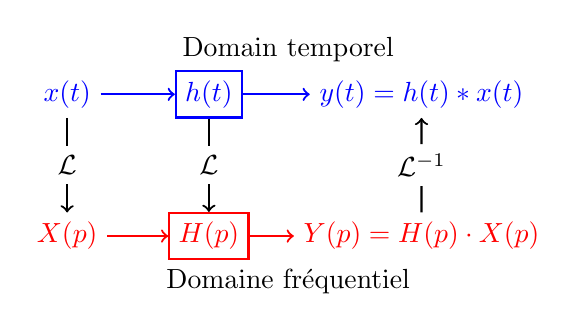
\begin{tikzpicture}

\begin{scope}[local bounding box=diagramme, scale=0.9, anchor=center, baseline]
    \node[blue] (x) at (0, 2) {$x(t)$};
    \node [draw, rectangle, thick, color=blue] (h) at (2, 2) {$h(t)$};
    \node[blue] (y) at (5, 2) {$y(t) = h(t) * x(t)$};
    \draw[->, thick, blue] (x) -- (h);
    \draw[->, thick, blue] (h) -- (y);
    
    \node (laplace1) at (0, 1) {$\mathcal{L}$};
    \node (laplace2) at (2, 1) {$\mathcal{L}$};
    \node (inverse_laplace) at (5, 1) {$\mathcal{L}^{-1}$};
    \draw[thick] (x) -- (laplace1);
    \draw[thick] (h) -- (laplace2);
    \draw[<-, thick] (y) -- (inverse_laplace);
    
    \node[red] (X) at (0, 0) {$X(p)$};
    \node [draw, rectangle, thick, color=red] (H) at (2, 0) {$H(p)$};
    \node[red] (Y) at (5, 0) {$Y(p) = H(p) \cdot X(p)$};
    \draw[->, thick, red] (X) -- (H);
    \draw[->, thick, red] (H) -- (Y);
    
    \draw[->, thick] (laplace1) -- (X);
    \draw[->, thick] (laplace2) -- (H);
    \draw[thick] (inverse_laplace) -- (Y);
\end{scope}
\node at (diagramme.north) [above] {Domain temporel};
\node at (diagramme.south) [below] {Domaine fréquentiel};
    
\end{tikzpicture}
    \caption{Source : \url{https://commons.wikimedia.org/wiki/File:Time_and_frequency_domains.svg?uselang=fr}}
\end{figure}

\[
\mathcal{L}(f \ast g) = \mathcal{L}(f) \mathcal{L}(g)
\]
